\section{Introducción}
En esta sección se comentan las herramientas y el entorno de desarrollo utilizado para la práctica, así como algunos detalles acerca de la preparación de los datos.

\subsection{Herramientas y entorno}

Se ha optado por utilizar bibliotecas disponibles públicamente, que implementan los algoritmos necesarios para la práctica. El entorno de desarrollo elegido ha sido un Jupyter Notebook en \textit{Google Colab}, haciendo uso de las funcionalidades de \textit{TensorFlow} y \textit{Keras}.

Esta elección se debe a su acceso gratuito a potentes recursos de computación como GPUs y TPUs, lo que acelera el entrenamiento de modelos complejos. Además, Colab ofrece un entorno preconfigurado y una integración fluida con Google Drive, lo que simplifica el almacenamiento de los conjuntos de datos de las imágenes.

\subsection{Preparación de los datos}

El objetivo es la implementación de redes neuronales para la identificación (o clasificación) correcta de dígitos en el conjunto de imágenes MNIST.

Antes de nada, se han definido cuatro funciones: las dos primeras (\autoref{fig:function-load-imgs}) se encargan de abrir los ficheros \texttt{train-images.idx3-ubyte} y \texttt{t10k-images.idx3-ubyte}, que contiene las imágenes para el entrenamiento y las pruebas respectivamente, mientras que las dos últimas (\autoref{fig:function-load-labels}) sirven para cargar las etiquetas correspondientes a los dos conjuntos de imágenes (\texttt{train-labels.idx1-ubyte} y \texttt{t10k-labels.idx1-ubyte}).

\begin{figure}[H]
	\centering
	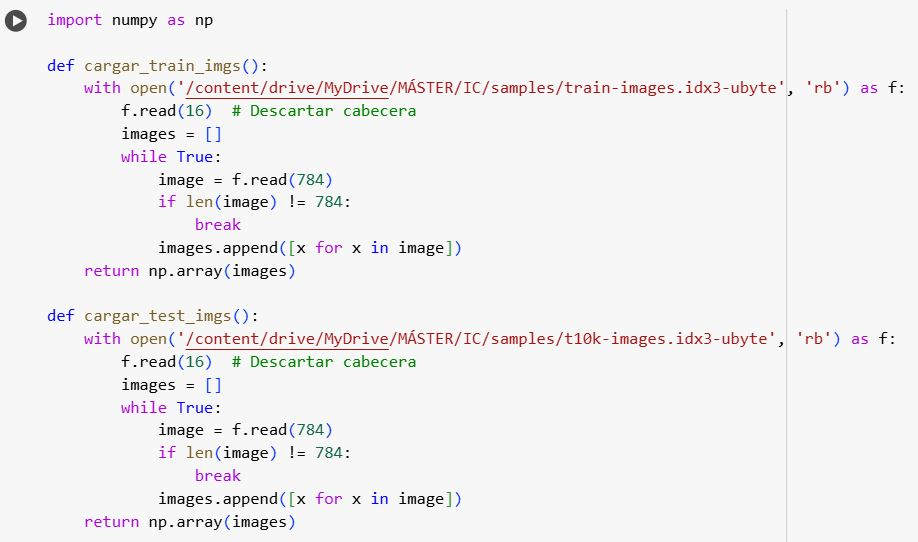
\includegraphics[width=0.7\textwidth]{imgs/function-load-imgs.JPG}
	\caption{Funciones para cargar las imágenes de entrenamiento y prueba}
	\label{fig:function-load-imgs}
\end{figure}

\begin{figure}[H]
	\centering
	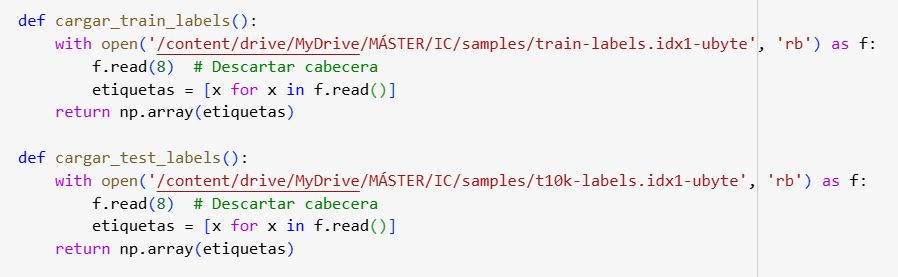
\includegraphics[width=0.7\textwidth]{imgs/function-load-labels.JPG}
	\caption{Funciones para cargar las etiquetas de los conjuntos de imágenes}
	\label{fig:function-load-labels}
\end{figure}

Una vez definidas las funciones anteriores, se llaman para cargar los datos. A continuación, se preprocesan las imágenes de entrenamiento y prueba normalizándolas, dividiendo sus valores de píxel por 255.0, lo que escala los valores al rango [0, 1]. Las etiquetas de ambos conjuntos se convierten a formato categórico utilizando \texttt{to\_categorical} con 10 clases, lo que transforma las etiquetas en vectores one-hot adecuados para la clasificación multiclase.

Finalmente, las imágenes de entrenamiento y prueba se reestructuran con la función \texttt{reshape} para tener dimensiones de 28x28 píxeles y un único canal (blanco y negro), preparando los datos en el formato requerido para ser ingresados en las redes neuronales. Estos pasos vienen implementados en la \autoref{fig:preprocessing}.

\begin{figure}[H]
	\centering
	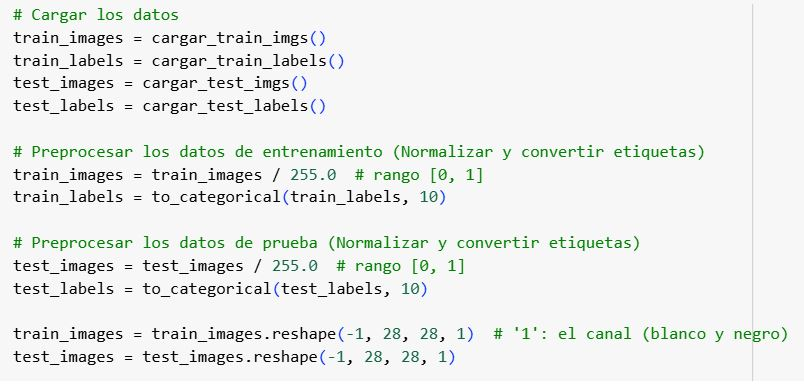
\includegraphics[width=0.7\textwidth]{imgs/preprocessing.JPG}
	\caption{Preparación de los conjuntos de datos}
	\label{fig:preprocessing}
\end{figure}

\subsection{Metodología}

Se va a seguir la siguiente metodología para cada red neuronal a implementar:

\begin{enumerate}
	\item \textbf{Creación del modelo}: se crea un modelo secuencial utilizando la clase \texttt{Sequential} de \textit{Keras}. Este modelo consiste en una pila lineal de capas que se añaden en orden.
	\item \textbf{Compilación del modelo}: se compila el modelo, pudiendo configurar el optimizador (como \texttt{adam}), la función de pérdida (como \texttt{categorical\_crossentropy}) y las métricas de evaluación (como \texttt{accuracy}, para monitorizar la precisión del modelo).
	\item \textbf{Entrenamiento del modelo}: \texttt{model.fit()} entrenará el modelo con los datos de entrenamiento, pudiendo indicarle el número de épocas (\texttt{epochs}), el tamaño de lotes (\texttt{batch\_size}) y el nivel de detalle de las salidas por consola (\texttt{verbose}).
	\item \textbf{Cálculo del tiempo de entrenamiento}: utilizando \texttt{time.time()} para registrar los tiempos de inicio y final del entrenamiento y así poder calcular la duración total.
	\item \textbf{Evaluación del modelo}: se evalúa el rendimiento del modelo tanto en el conjunto de entrenamiento como en el de prueba, teniendo en cuenta la pérdida y precisión, y pudiendo indicar con \texttt{verbose} cuántos detalles de la evaluación mostrar por la consola.
	\item \textbf{Cálculo del porcentaje de error}: se calculan los errores de entrenamiento y de prueba mediante la expresión $error\% = 100 - accuracy * 100$. Estos errores se imprimen como porcentajes con dos decimales, proporcionando una medida clara de las tasas de fallo del modelo en ambos conjuntos de dato.
	
\end{enumerate}

Los tres últimos pasos anteriores vienen descritos en la \autoref{fig:show-results}.

\begin{figure}[H]
	\centering
	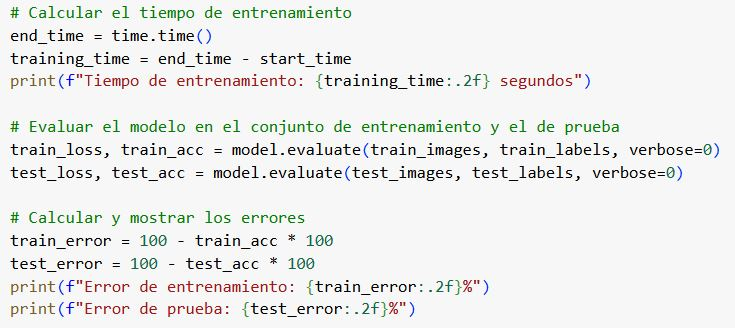
\includegraphics[width=0.7\textwidth]{imgs/show-results.JPG}
	\caption{Fragmento de código para imprimir los resultados del modelo}
	\label{fig:show-results}
\end{figure}
